\section{Results, convergence monitoring, and model checking}
\label{results_convergence_checking}


\subsection{Convergence monitoring}
\label{subsection_convergence}

Before making inferences using posterior simulations generated by an MCMC algorithm 
it is essential to check for evidence of convergence to the target distribution. Although this 
process is not an exact science, there is no shortage of literature on the topic of monitoring 
convergence for MCMC and other iterative simulation algorithms. The various convergence 
diagnostics used below are introduced informally. Formal definitions, computational details, 
and recommended best practices can be found in \citeA{gelman_handbook_2011}, 
\citeA{gelman_bayesian_2013}, and \citeA{stan_development_team_stan_2015}.

Eight randomly initialized chains of 2000 iterations (including a warmup period of 1000 
discarded draws) were simulated.\footnote{Newcomers to HMC, NUTS, and Stan are 
often surprised by how few iterations are typically required, as it is not uncommon for 
Gibbs (and poorly tuned M-H) samplers to require hundreds of thousands of iterations 
to converge. Simpler models fit in Stan often require only hundreds of iterations, including 
warmup. This is due in large part to the advantages of HMC discussed in \ref{stan_intro}, in
particular the suppression of random walk behavior leading to more efficient exploration
of the parameter space.} 

\begin{figure}[t]
\centering
	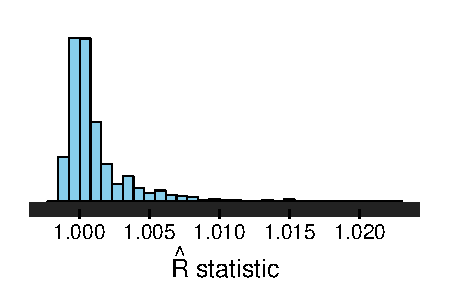
\includegraphics[scale=0.7]{sections/figs/rhat}
	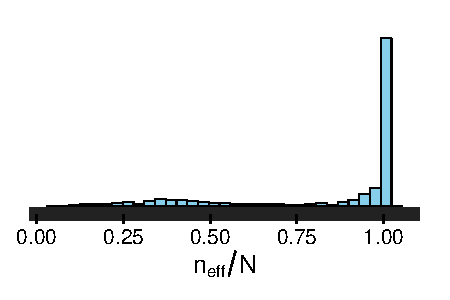
\includegraphics[scale=0.7]{sections/figs/neff}
	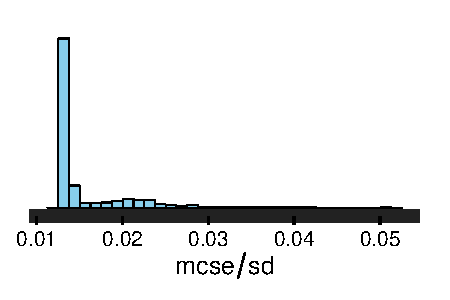
\includegraphics[scale=0.7]{sections/figs/mcse}
\caption{Distributions of diagnostics computed from the MCMC draws. 
From left to right: \newline ({\bf a}) Potential scale reduction factor $\hat{R}$ \newline ({\bf b}) 
Ratio of effective sample size to total sample size ($n_{\it eff}/N$) \newline ({\bf c}) Ratio of 
Monte Carlo error to posterior standard deviation ($mcse/sd$)}
\label{fig:ck_diagnostics}
\end{figure}

In Figure~\ref{fig:ck_diagnostics}, panel ({\bf a}) shows the distribution of the estimates of 
the potential scale reduction statistic $\hat{R}$  \shortcite{gelman_rhat_1992}. The $\hat{R}$ 
statistic is a comparison of the variance of the simulations within individual chains to that of 
the simulations when chains are pooled. Here, the distribution of $\hat{R}$ shows that for 
all parameters the value is approximately one, indicating that little would be gained by running 
longer chains \shortcite{gelman_handbook_2011}. 

Panel ({\bf b}) shows the distribution of the ratio of effective sample size to the number of 
iterations ($n_{\it eff}/N$). Roughly speaking, $n_{\it eff}$ is an estimate of the number of 
{\it independent} draws from the posterior distribution that would have the same expected 
variance as the $N$ {\it dependent} draws actually obtained from the 
Markov chains. In the absence of autocorrelation $n_{\it eff} = N$, and so the ideal value of the ratio is one. 
In this case $n_{\it eff}/N$ is sufficiently large -- it is at least 20\% for all parameters -- and 
for most parameters the ratio is close to one, a reflection of Stan's efficiency. 


The distribution of the ratio of Monte Carlo error to the estimated standard 
deviation ($mcse/sd$) is shown in panel ({\bf c}) of Figure~\ref{fig:ck_diagnostics}. 
Monte Carlo error is a measure of imprecision due to approximating 
the posterior distribution by the MCMC simulations. As the number of iterations increases 
$mcse$ tends toward zero and the standard deviation of the draws converges to the posterior 
standard deviation. In this case, for all parameters 
the relative error $mcse/sd$ is less than five percent, which, for the inferential goals of this 
analysis, is negligible. For instance, Figure~\ref{fig:ck_example_posterior} shows the estimated 
posterior density for the parameter corresponding to bias towards the majority party in the 79th 
congress.\footnote{There is nothing special about the 79th congress for this purpose. A single 
congress was chosen at random to use as an example.} The posterior is approximately Gaussian, 
with mean and standard deviation of roughly $0.054$ and $0.037$, respectively. The 
estimated $mcse$ is $0.0007$, which is inconsequential when compared to the uncertainty about 
the parameter in the posterior distribution.   


\begin{figure}[h]
\centering
	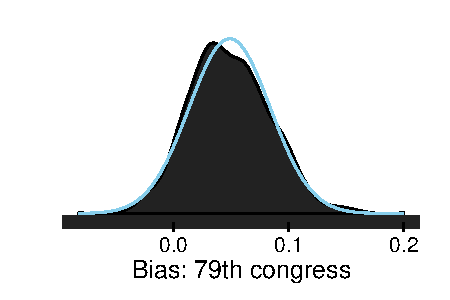
\includegraphics[scale=0.75]{sections/figs/example_posterior}
\caption{Posterior kernel density estimate for bias towards the majority party in the 79th congress. 
Normal density curve in blue.}
\label{fig:ck_example_posterior}
\end{figure}


%DEPENDENCE PLOT?
%
%
%\begin{figure}[h]
%\centering
%	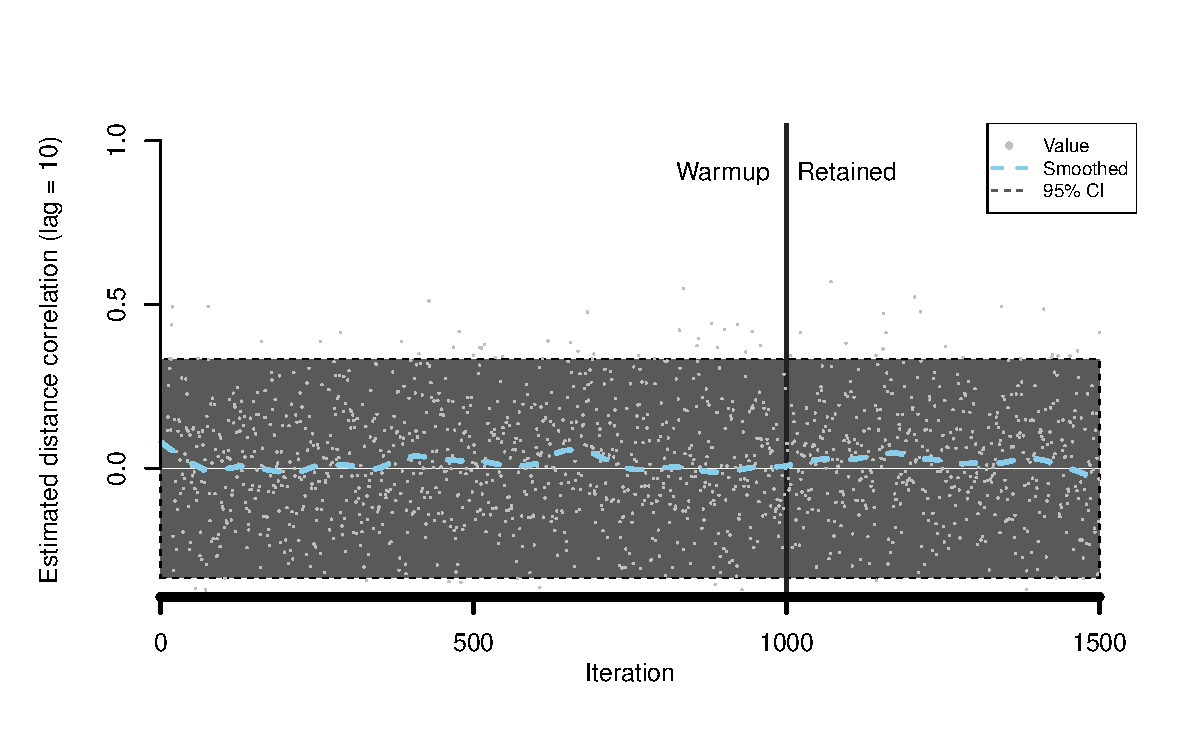
\includegraphics[scale=0.75]{sections/figs/ck_dependence}
%\caption{Estimated distance correlation among the eight chains. At a lag of 10 the draws are essentially independent. }
%\label{fig:ck_dependence}
%\end{figure}
%

In addition to the diagnostics discussed above, trace plots for all parameters were also 
examined as well as additional quantities specific to HMC and NUTS.\footnote{For example, 
checking that the tree depth used by NUTS is well below the user-specified maximum, ensuring 
that there are no post-warmup leapfrog iterations with diverging error, etc. These are explained 
in greater detail in \citeA{stan_development_team_stan_2015}.}


\subsection[Estimates]{Estimated bias toward the majority party}
\label{results}

\subsubsection{Comparing the results}

Figure~\ref{fig:ck_bias} (p.~\pageref{fig:ck_bias}) juxtaposes the estimates of 
bias towards the majority party over time from Cox and Katz's analysis and the reanalysis 
using the Bayesian STAR model.

\begin{figure}
\centering
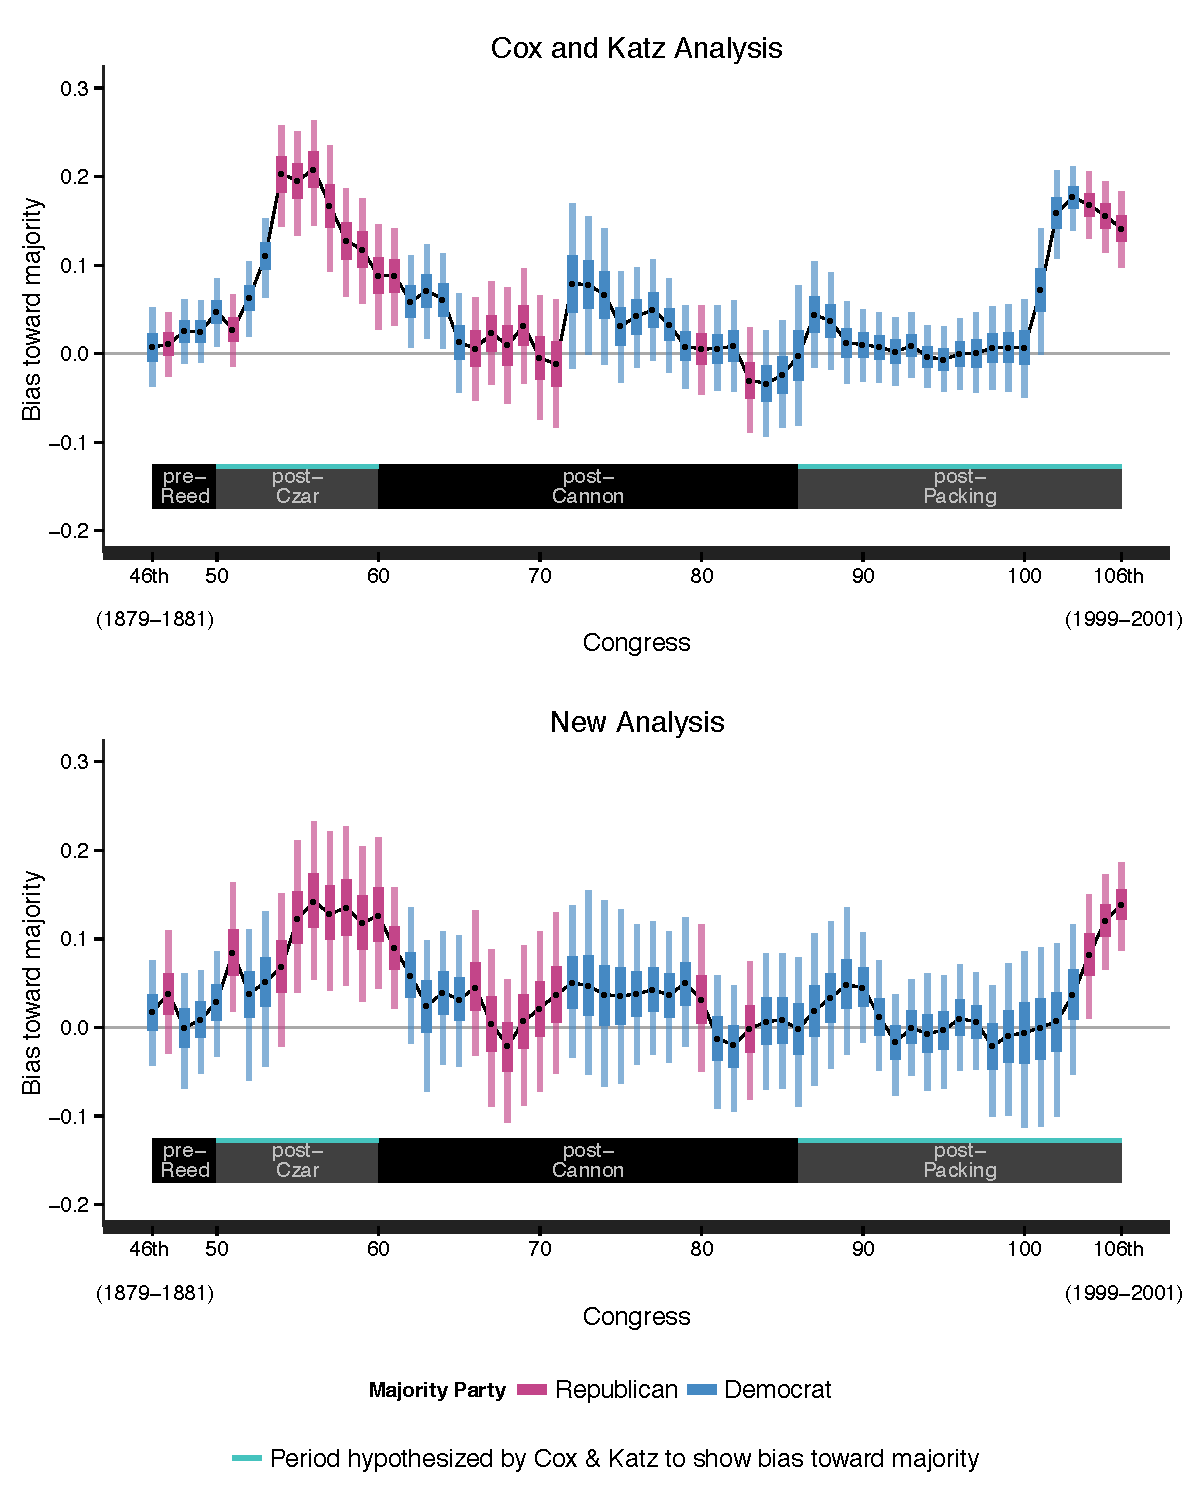
\includegraphics[scale=0.75]{sections/figs/ck_replication_new}
\caption{Estimated bias toward the majority party by Congress in 
Cox and Katz's analysis (top) and the Bayesian reanalysis (bottom). 
The thin and thick vertical segments represent 95\%  and 50\%
intervals, respectively.  The black line connects medians.
To produce the graph on top Cox and Katz's original analysis was 
replicated (see Figure 3 in Cox and Katz (2007)).}
\label{fig:ck_bias}
\end{figure}

Immediately noticeable is that the new estimates have greater 
uncertainties, which is to be expected due to the potential for Cox and Katz's method to 
produce overly precise estimates  (see section \ref{subsection_methods}). The new results 
do provide some support for the hypothesis of bias during the post-czar and post-packing 
periods; the evidence is much weaker than that found by Cox and Katz, but the finding 
of bias toward the Republican majority in the latter half of the post-czar period holds up. 

When compared to Cox and Katz's results, the hierarchical Bayesian STAR model estimates 
a more believable trend in bias over time. This can be seen clearly by comparing the curves 
in Figure~\ref{fig:ck_bias}. The smoothing prior shrinks each individual estimate slightly 
towards its neighbors -- the amount of smoothing is related to the hierarchical variance 
hyperparameter -- and all estimates are regularized to the common prior mean, which helps 
avoid overfitting the data, while still allowing for substantial movement between Congresses 
if strongly supported by the data. Although both sets of results agree on the direction of the 
estimates in the post-czar period, while the Cox and Katz estimates show signs of overfitting 
the data the new estimates are less volatile. 


\subsubsection{Different interpretations}

Although Figure~\ref{fig:ck_bias} appears to be showing two versions of the same plot with
slightly different estimates, Cox and Katz's results (obtained by maximum likelihood estimation) 
and the results from the Bayesian model must be interpreted differently. The former are point estimates 
and confidence intervals, whereas the full Bayesian model provides an estimate of the marginal posterior 
{\it distribution} for each parameter. That is, the estimates obtained from the Bayesian model are the 
distributions themselves; presenting the results as point estimates and intervals is simply convenient for 
making comparisons to Cox and Katz's results. 

In the classical approach taken by Cox and Katz, a single value is obtained for each parameter and 
assessed in relation to infinitely many confidence intervals constructed from infinitely many hypothetical 
datasets. While in many situations it is possible to imagine repeating an experiment (e.g. coin flipping), 
such an interpretation makes less sense in the context of the historical events of interest to this analysis. 
For each confidence interval obtained from Cox and Katz's analysis, all that can be said is that it either 
contains the (theoretical) true parameter value or it does not. This is a consequence of taking the 
philosophical position that the parameter is fixed while the data and interval bounds are 
random variables. 

On the contrary, from the Bayesian perspective the parameter is treated as a random variable while 
the data and interval bounds are fixed. As a result, the estimates from the  Bayesian model have a 
more intuitive interpretation. Conditional on the model and data, there is a $p\%$ probability that the 
(theoretical) true value of the parameter lies in the $p\%$ interval. 

\subsubsection{Problems with statistical significance}

Cox and Katz present their results in terms of statistical significance, which is problematic 
for several reasons. First, if the reported 
standard errors understate the uncertainty in their estimates -- and this is presumably the case, as 
emphasized above and in \ref{subsection_methods} -- then the results will be biased towards
statistical significance (regardless of the threshold for determining significance). Second, in several
cases, the difference between bias toward the majority being statistically significant in Congress $t$ 
and not significant in Congress $t + 1$ (or vice-versa) is not itself statistically significant. 

One such example is given in Figure~\ref{fig:ck_signif}, which shows Cox and Katz's 
point estimates and 95\% intervals for bias in the 100th and 101st Congresses. 
The estimates (plus or minus one standard error) are $b_{100} = 0.0065 \pm 0.029$ 
and $b_{101} = 0.071 \pm 0.034$. Assuming the 95\% threshold for statistical significance 
standard in the social sciences and used by Cox and Katz, $b_{101}$ is statistically significant 
but $b_{100}$ is not. Though it is then tempting to conclude that one is signal while the other 
is indistinguishable from noise, note that the difference between the two is 
$0.0645$ with a standard error of $0.045$ and thus not close to statistically significant. 
The general point is that nonsignificant changes can correspond to large changes 
in significance levels.\footnote{A more detailed explanation of this issue -- which is not unique to this 
example -- and its potential consequences can be found in Chapter 2 of \citeA{gelman_arm_2007}.} 


\begin{figure}
\centering
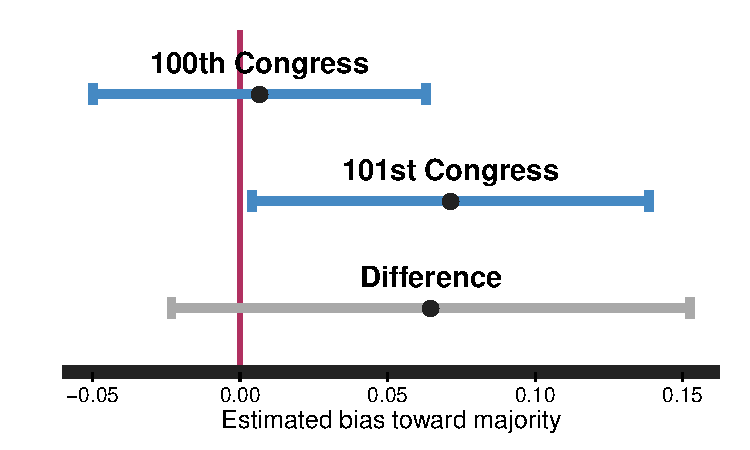
\includegraphics[scale=0.75]{sections/figs/ck_signif}
\caption{An example of when the difference between statistically significant and nonsignificant is 
not itself statistically significant.}
\label{fig:ck_signif}
\end{figure}

\subsubsection{Problems with rolling windows}

As discussed in \ref{subsection_methods}, Cox and Katz's results comprise estimates taken 
from 61 separate models (one for each Congress). This results in the data for each Congress 
$t$ being reused in up to six of the 60 models besides the model for Congress $t$ itself. It also 
entails the exclusion of all data from Congresses outside each window. Furthermore, the 
choice of using rolling windows of seven Congresses ($t \pm 3$) is also somewhat arbitrary. 

The curves in Figure~\ref{fig:ck_hypothetical} (p.~\pageref{fig:ck_hypothetical}) show the 
results Cox and Katz would have found had they chosen narrower or wider windows. As the 
set of Congresses included in each model grows, the resulting curve necessarily becomes 
smoother because Cox and Katz's method is less and less distinguishable from simply 
estimating a common bias parameter for all Congresses (that is, assuming no variation in 
bias over time). Conversely, the single Bayesian model allows for bias in each Congress to 
depend on neighboring Congresses while using the entire dataset only once, obviating the 
need to dubiously subset the data. 

\begin{figure}
\centering
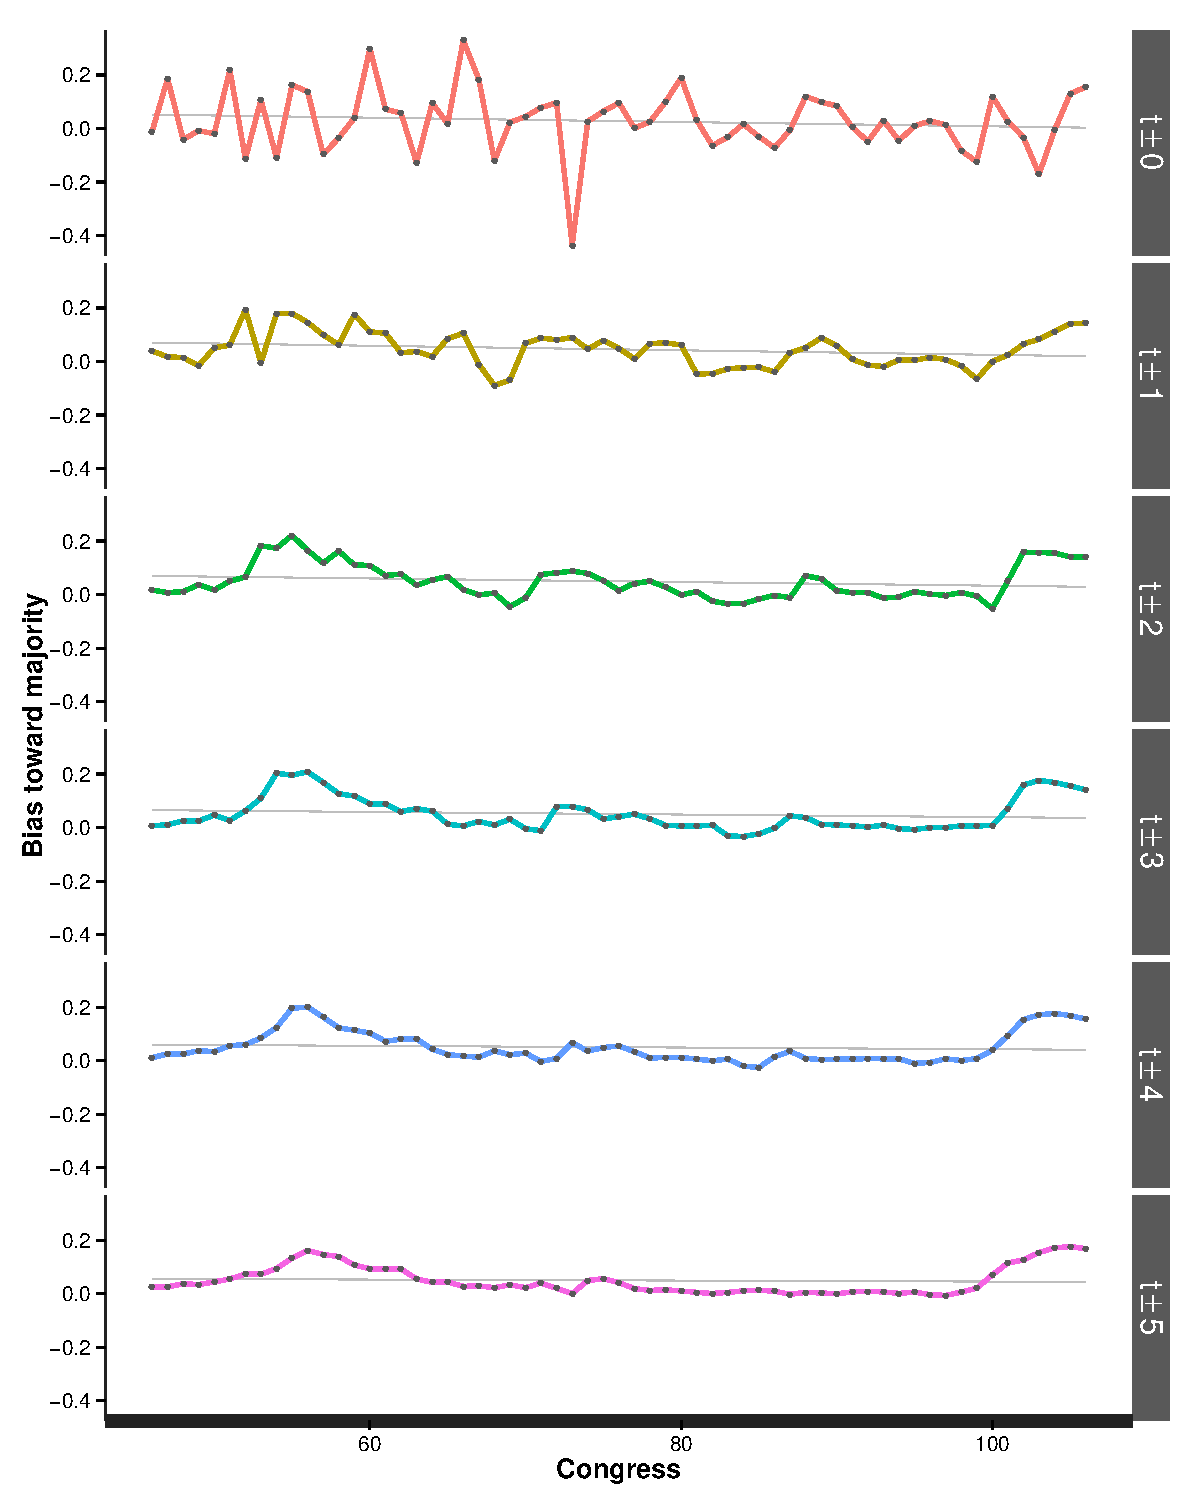
\includegraphics[scale=0.75]{sections/figs/ck_hypothetical}
\caption{Replications of Cox and Katz's results but changing the number of Congresses 
included when estimating each point. The top panel corresponds to estimating bias in each 
Congress $t$ using only data from time $t$ (i.e., $t \pm 0$). In each subsequent panel the 
set of Congresses is expanded by one in both directions. The bottom panel corresponds to 
using $t \pm 5$. The analysis presented in \protect\citeA{cox_gerrymandering_2007} is the 
panel for $t \pm 3$. The horizontal gray lines are the estimates obtained by completely 
pooling the data from all Congresses. Error bars are excluded so that differences in the 
smoothness of the curves are more perceptible.}
\label{fig:ck_hypothetical}
\end{figure}




\subsection{Model checking: graphical posterior predictive checks}
\label{subsection_model_checking}

Graphical posterior predictive checking is a valuable tool for examining how well the proposed model 
fits the available data \shortcite{gelman_bayesian_2013}. The idea is simple: if the model is a good fit 
then it should be possible simulate data from the model that resembles the observed data. Let $\Theta$ 
denote all parameters (including hyperparameters) in the hierarchical model. Following 
 \citeA{gelman_bayesian_2013}, $y^{\it rep}$ will be used to denote a replication of $y$ from the model.\footnote{\citeA{gelman_bayesian_2013} distinguishes between $y^{rep}$ and $\tilde{y}$. The former 
 makes use of the same explanatory variables/predictors $x$ used to estimate $\Theta$, while the latter 
 refers predictions of future $y$ using potentially different variables $\tilde{x}$ (e.g. after collecting more data).}

For each draw of the parameters $\Theta$ from the posterior distribution $p(\Theta | y)$ an entire set 
of data $y^{\it rep} $ is simulated from the posterior predictive distribution,

\begin{equation*}
 p(y^{\it rep} | y) = \int p(y^{\it rep}, \Theta | y) d\Theta = \int p(y^{\it rep} | \Theta) p(\Theta | y) d\Theta,
\end{equation*}

\noindent which can be viewed as the likelihood for the new data $y^{\it rep}$ averaged over 
the posterior distribution for the parameters $\Theta$.\footnote{For instance, if $y$ is an $N$-vector 
and there are $D$ draws of $\Theta$ from $p(\Theta | y)$, then $D$ replicated data sets $y^{rep}$ 
will be simulated, each of which is also an $N$-vector.}

The twelve histograms in Figure~\ref{fig:ck_pp_hists} (p. \pageref{fig:ck_pp_hists}) show the 
distribution of the observed data $y$ -- the number of roll-call votes won by the majority party 
-- alongside eleven replicated data sets $y^{\it rep}$ randomly selected from all of the posterior 
predictive replications. This is a casual but informative comparison; it is an easy way of checking 
for inconsistencies due to poor model fit. In this case it shows that indeed the observed data are 
plausible under the posterior predictive distribution implied by the model. 
Figure~\ref{fig:ck_pp_nWins_hists} (p. \pageref{fig:ck_pp_nWins_hists}) is similar to 
Figure~\ref{fig:ck_pp_hists} but shows the distribution of $y^{\it rep}$ by Congress. Again it is 
evident that the observed data are consistent with the posterior predictive distribution. Finally, 
Figure~\ref{fig:ck_pp_test_statistics} (p. \pageref{fig:ck_pp_test_statistics}) shows the distributions 
of the mean and standard deviation over all replications, which nicely fit the observed values of 
these statistics in the data. 

% Should probably do pp checks after aggregating over the sub periods for each congress.  

\begin{figure}[h]
\centering
	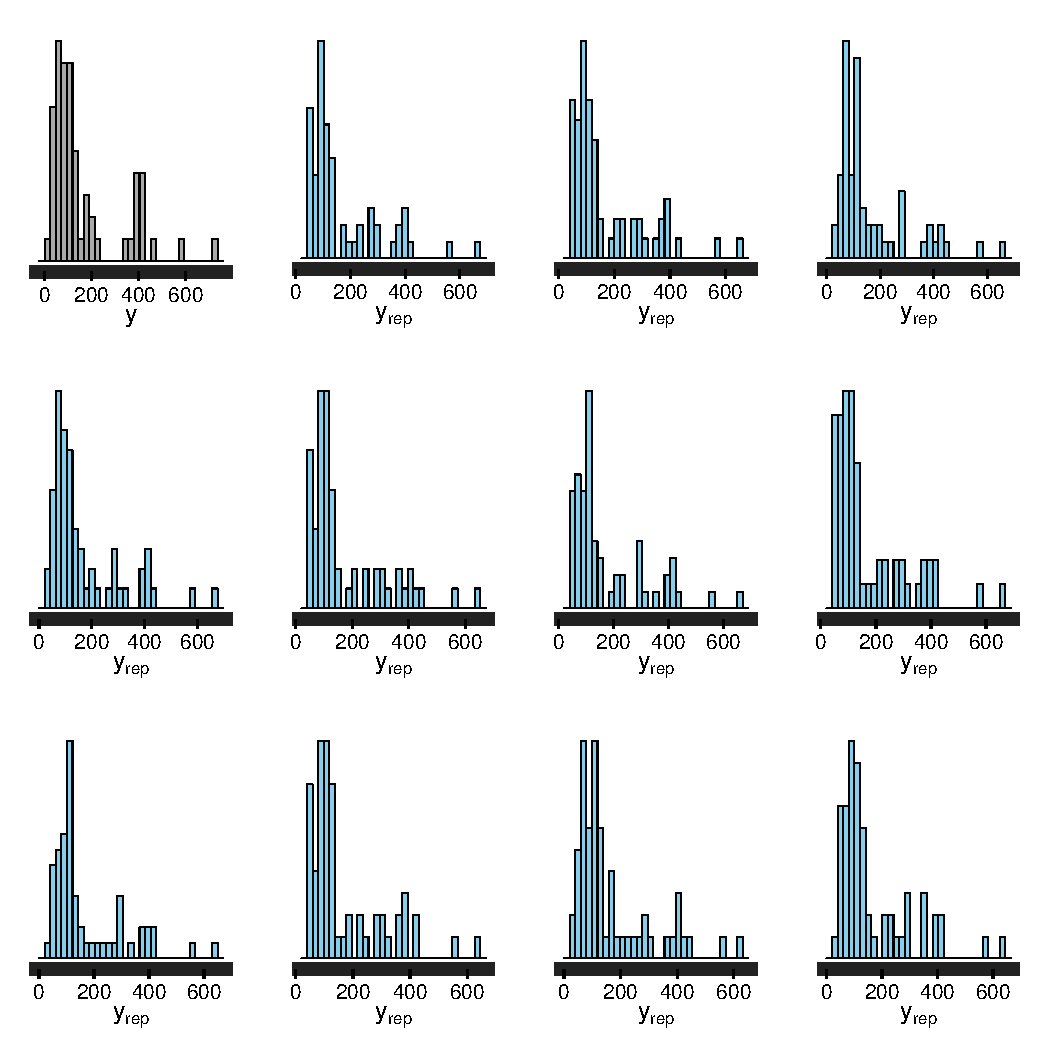
\includegraphics[scale=0.6]{sections/figs/ck_pp_y_vs_yrep_hists}
\caption{Replications from posterior predictive distribution vs. observed data}
\label{fig:ck_pp_hists}
\end{figure}

\begin{figure}[h]
\centering
	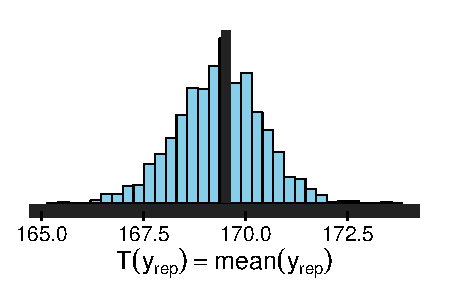
\includegraphics[scale=0.75]{sections/figs/test_stats_mean}
	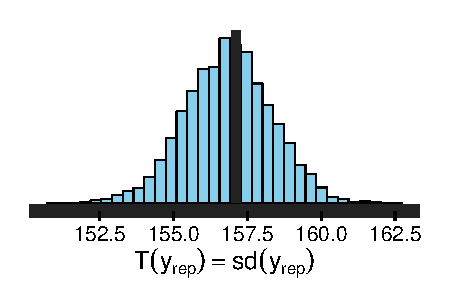
\includegraphics[scale=0.75]{sections/figs/test_stats_sd}
\caption{Distributions of test statistics $T(y_{rep})$. The vertical bar is the observed value $T(y)$.}
\label{fig:ck_pp_test_statistics}
\end{figure}

\begin{figure}
\centering
	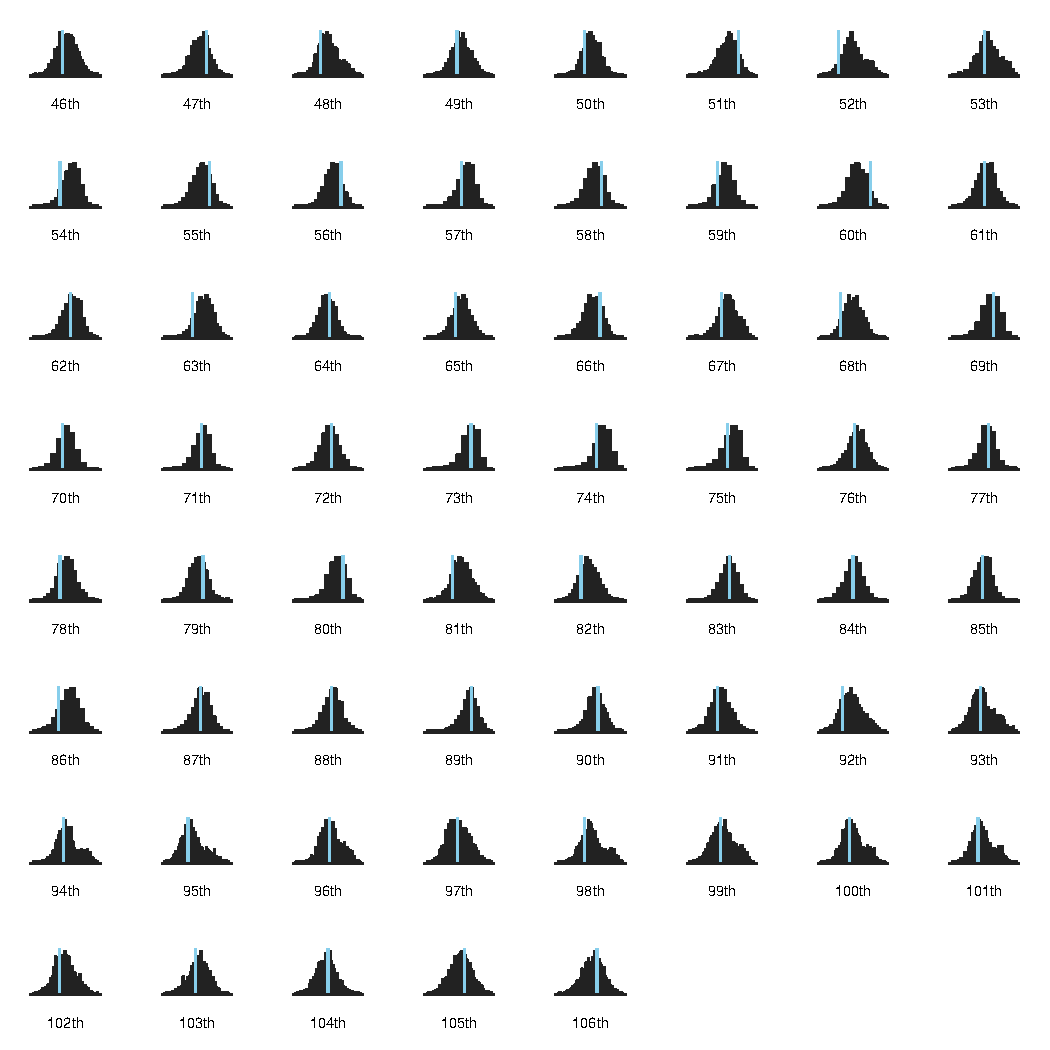
\includegraphics[scale=0.8]{sections/figs/ck_pp_nWins_hists}
\caption{Distributions of $y^{\it rep}$ by Congress. Vertical lines show observed values from the data.}
\label{fig:ck_pp_nWins_hists}
\end{figure}
